
\appendix
\section{User Interface Designs}
\label{sec:ui_designs}

\subsection{ Partridge Query Interface}


Figure \ref{fig:ui_mockup} shows the user interface that will be utilised to
search and query Partridge's corpus. 

The query form shows two main sections: Filters and Keywords. 

Filters can be used to show a large set of papers where the user is unsure of
what to search for. Users will be able to look for papers by type and topic as
discussed above. The paper result filter has not been included in this diagram.
However, it is expected that a drop down menu for result type would be included
in the filters section of the form.

Keywords allows the user to look for a set of keywords that is specifically
within a CoreSC concept for a paper. For example, the reader may want to find
experiments that use a server farm to do lots of calculations. Therefore, they
would enter ``Server Farm" as their keywords and chose ``Method" from the paper
section. The user then adds this to the set of keyword queries in the table
below the text field with the add button.

Once a user has configured both filters and keywords to their preferences, they
click the search form to run the search itself.

Other notable features on this mockup include a list of most recent searches.
This helps the user to understand how to use Partridge and gives them some
suggestions for what they might search for. Similar listings are provided for
the most popular papers in the Partridge database and the most recent papers
added to the system.

\begin{figure}[!ht]
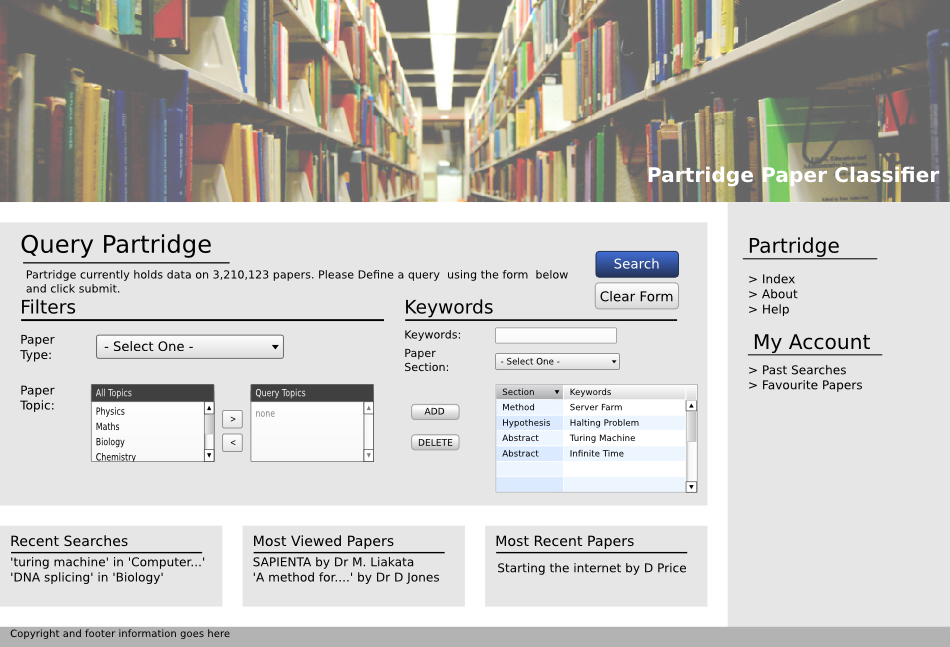
\includegraphics[width=\textwidth]{images/mockup_1.png}
\caption{User interface design for querying Partridge}
\label{fig:ui_mockup}
\end{figure}


\section{System Process Diagrams}
\label{sec:system_diagrams}

This section documents the system process diagrams that have been produced. The
first completed diagram shows how a paper will be added to Partridge and the
actions that will be carried out upon it.

\subsection{Adding a Paper to Partridge}

\begin{figure}[!ht]
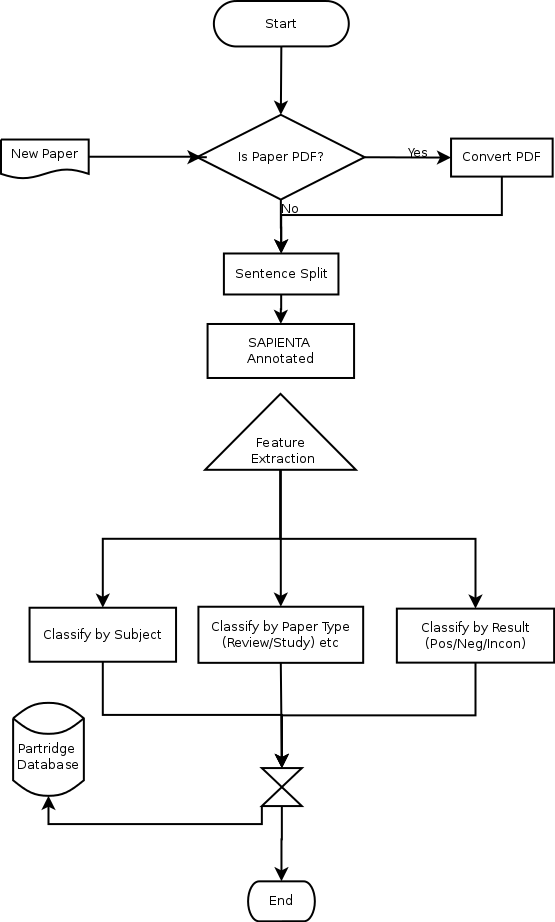
\includegraphics[width=0.75\textwidth]{images/PaperAddedProcess.png}
\caption{The process of adding a new paper to Partridge}
\end{figure}

The system starts off by converting the document to XML from PDF if necessary
through the use of the PDFX tool provided by Manchester University. A sentence
splitting tool is then used to parse the resulting document and separate the
sentences.

Once the sentences have been split, Maria's SAPIENTA tool is used to annotate
each sentence to determine which of the core scientific concepts it covers.
This information is stored back in the XML file with the document.

After this, feature extraction is carried out upon the document to find useful
features for the following classification tasks:

\begin{enumerate}
\item Paper topic/subject -i.e. is the paper a biology paper or a computer science paper?
\item Type of paper - i.e. is the paper a case study, an experiment or a literature review?
\item Paper result - i.e. did the paper have a positive, negative or inconclusive result?
\end{enumerate}

These classifiers are then run (they could potentially be run in parallel if
processing power is available) to determine the paper's class for each
classifier respectively. The data gathered along with any paper metadata
captured such as title, author, date, institute etc are then stored in the
database.


\section{Email for CRFSuite}
\label{sec:crfemail}
\begin{verbatim}
Hi All,

I'm trying to build CRFSuite's python extension 
(http://www.chokkan.org/software/crfsuite/) on an Arch Linux 64-bit 
environment using Swig 2.0.8 (PCRE enabled).

When I run SWIG, I get the following output:

<<OUTPUT OMITTED FOR BREVITY>>

Full output available at http://sourceforge.net/mailarchive/message.php?msg_id=30024209

As far as I can see, all of these problems stem from this declaration in 
the SWIG input file (http://pastebin.com/9JipJ1C1):
%template(ItemSequence) std::vector<CRFSuite::Item>;

I've had a look around on google and on this mailing list and the only 
other "cannot copy typemap" errors I've encountered have been where 
people have excluded the std namespace in favour of a 'using' statement. 
As you can see, this example uses absolute class names so that isn't the 
issue here. I haven't had any luck contacting the software maintainer 
for CRFSuite yet either.

As you might expect, if I continue to compile the extension without 
heeding these errors, when I try to make use of the ItemSequence object 
I get the following python error:
TypeError: in method 'ItemSequence_append', argument 2 of type 
'std::vector< CRFSuite::Item >::value_type const &'

I'm going to keep trying to sort this out and if I find the solution 
independantly, I'll make sure to post a follow-up email. However, if 
anyone else has any ideas about what might be happening here, please let 
me know.

Thanks,

James Ravenscroft
AI & Robotics Undergraduate
Aberystwyth University
\end{verbatim}


\section{Project Timeline}
\label{sec:timeline}

This table shows the projected timeline for the Partridge project. These
calculations were carried out under the assumption of 2 full days of work per
week on the project and one iteration equating to one month (28 days). There
will be 7 iterations in total and after each, a new version of Partridge will
be made available (except for iteration zero which is a research only
iteration).


\begin{figure}[htp] 
 \vspace{ -1cm }
 \centering{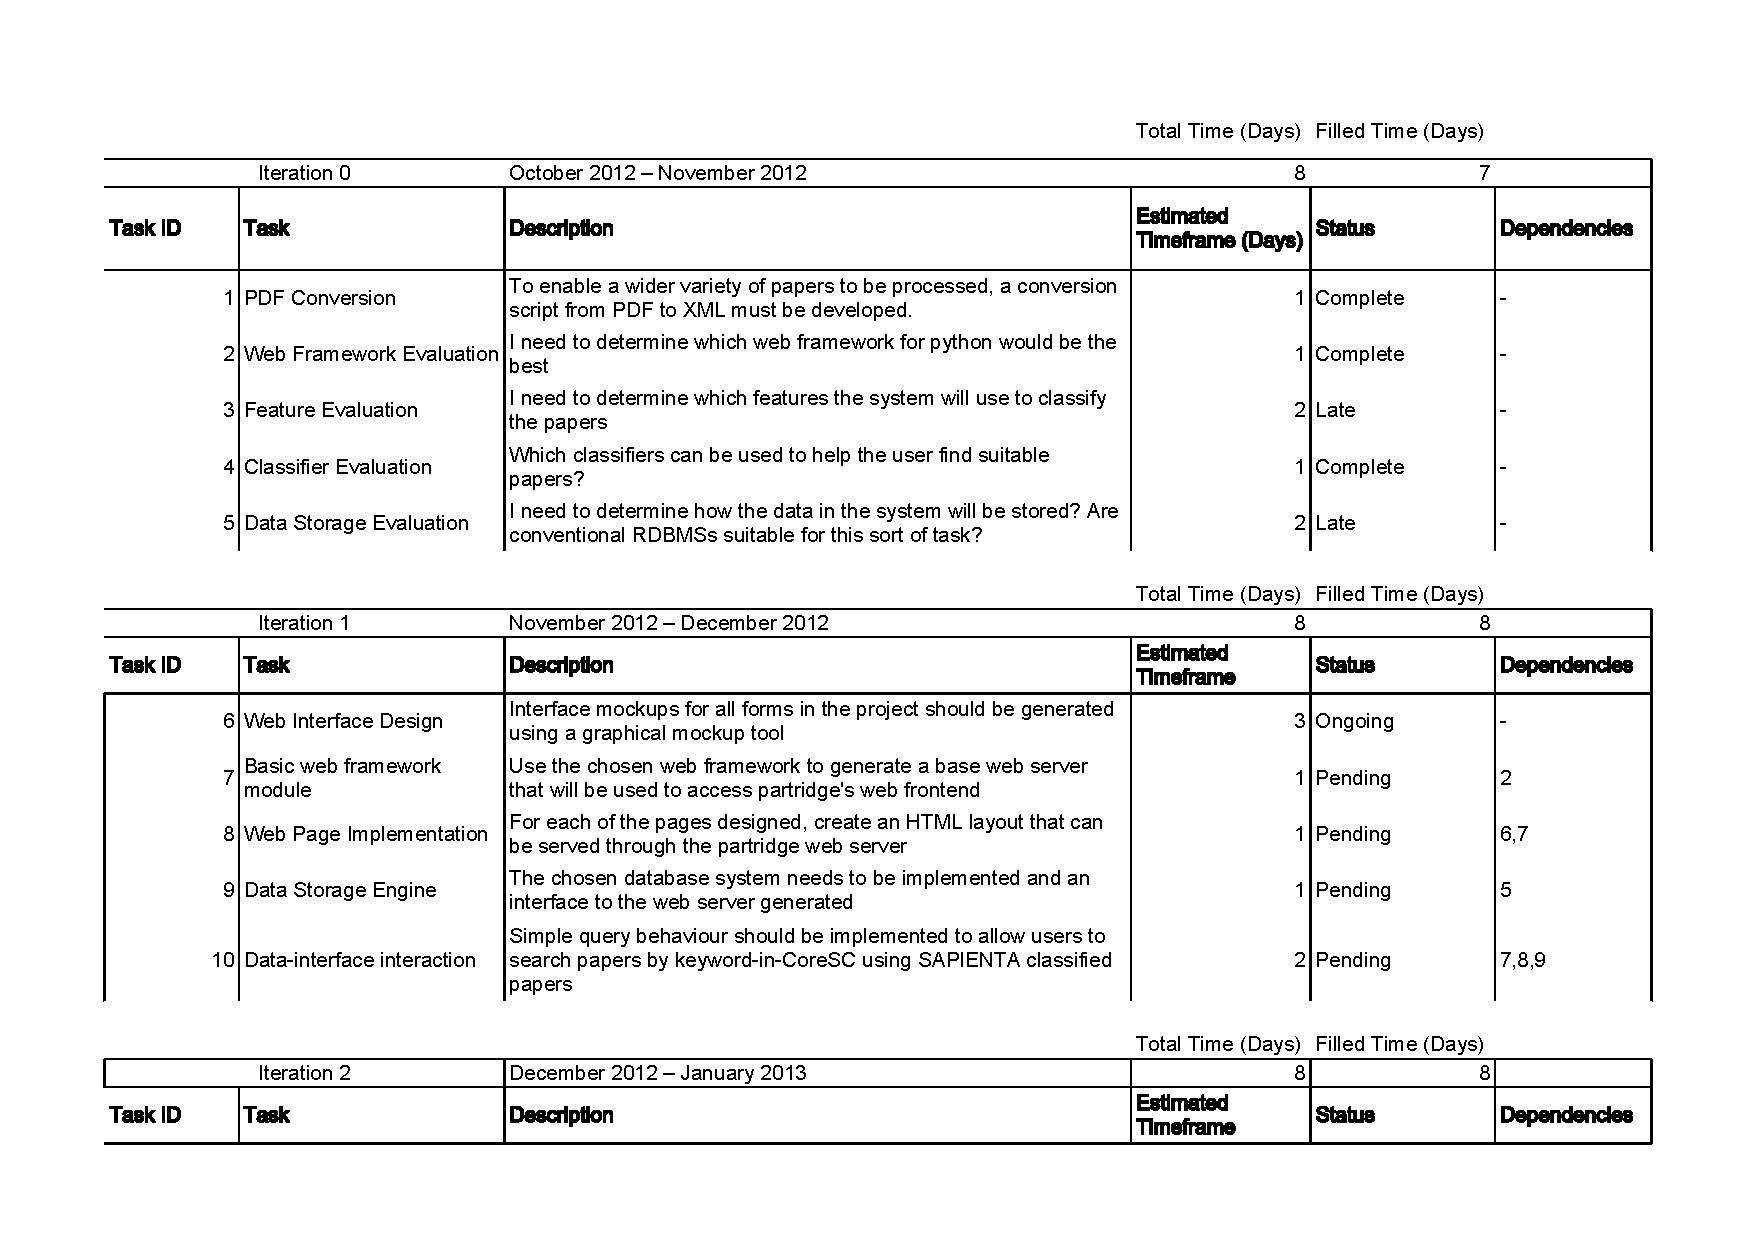
\includegraphics[scale=0.60,page=1]{../timeline.pdf}}
  
\end{figure}

\begin{figure}[!htp] 
 \centering{\includegraphics[scale=0.60,page=2]{../timeline.pdf}}
 \vspace{-2cm}
\centering{\includegraphics[scale=0.60,page=3]{../timeline.pdf}}
\end{figure}

\pagebreak
\section{Project Wiki}
\label{sec:wiki}

All pages from the Wiki are shown below with the exceptions of those pages
which have already been mostly featured in the document (UI Mockups and
Progress Diagrams and the project timetable are not shown in this section).

\subsection{ Notes 03/10/2012 }
\subsection{Meeting Notes from 03/10/2012}

\subsubsection{General topics}

\begin{itemize}
\item
  Talked about using research papers instead of books :-
\item
  copyright issues - mainly resolved because of Gutenburg project
\item
  processing issues - too much information to process quickly and
  realistically
\item
  Maria has some software for identifying sections in papers - could be
  used to help locate specific features
\item
  There are quite a few sources for papers that could be used for the
  project:
\item
  http://arxiv.org/
\item
  http://plosone.org/
\item
  Maria's papers are in XML format
\item
  Formatting may or may not be an issue - PDFs are a nightmare to parse
\end{itemize}

\subsubsection{Things to consider}

\begin{itemize}
\item
  What sort of recommendations for different sources might there be and
  how would these recommendations be extracted?
\item
  Feature engineering - what sorts of features might there be to pick
  out in the papers?
\item
  I need to have a read through the sentiment analysis paper that Maria
  has been working on
\item
  I need to have a play with the software for identifying sections in
  papers.
\end{itemize}

\subsubsection{Misc concerns}

\begin{itemize}
\item
  Decided that our weekly meeting should be Wednesdays at 3pm
\item
  Investigate setting up source control and a wiki (that's been done as
  you can tell)
\end{itemize}


\subsection{ Notes 10/10/2012 }
\subsection{Meeting Summary 10/10/2012}

\subsubsection{From Maria's notes}

\begin{itemize}
\item
  James has gone through papers and thinks would be more doable to work
  with papers than Books
\item
  James has found the XML format of PlosOne and ART/CoreSC corpus
\item
  Domain needs to be determined
\item
  Maria to send paper on sentiment analysis of citations
\end{itemize}

\subsubsection{Current features and recommendations}

\begin{itemize}
\item
  Analysis of results section - positive or negative result
\item
  Potentially look at writing styles of authors using syntactic analysis
\item
  Isolating terms within sections of papers (i.e.~find me papers where
  methodology x was used)
\item
  finer grain analysis of CoreSC categories
\item
  nltk python toolkit. What other toolkits? Would jerboa be any good?
\item
  common features for sentiment analysis
\end{itemize}

\subsubsection{Basic system design}

I have started a basic system design although it is very basic at the
moment. [Image Omitted]

\subsubsection{Background - Similar Systems and how they work}

\begin{itemize}
\item
  Google Scholar
\item
  Mendeley
\item
  Citeulike
\item
  Tweeting or `liking' on facebook.
\end{itemize}

\subsubsection{Reading}

\begin{itemize}
\item
  TF-IDF
\item
  Take a brief look at journal of negative results
\item
  `Bigrams + trigrams' and syntactic pattern finding
\item
  Common features used in NLP
\item
  Sentiment analysis of citations in papers
\item
  `Bag of words'
\end{itemize}

\subsubsection{Coding/practical research}

\begin{itemize}
\item
  Play some more with SAPIENTA
\item
  Implement a (La)TeX to SciXML or pubmed command-line tool.
\end{itemize}


\subsection{ Notes 19/10/2012 }
\subsection{Notes from Meeting 18/10/2012}

\subsubsection{General Comments}

\begin{itemize}
\item
  I need to decide on a domain for the project. It may be that papers on
  a varied selection of topics would be a good start
\item
  Decided on an agile development cycle with a basic program that is
  improved in `iterations'.
\item
  As part of testing the software, it may be possible to get other final
  year students to trial the engine and use it to make recommendations
  for their reading.
\item
  I need to investigate ways of analysing papers for syntactic patterns.
  This may be indicative of:

  \begin{itemize}
  \item
    Different authors' writing styles
  \item
    Different types of paper -i.e.~psychology vs physics
  \end{itemize}
\end{itemize}

\subsubsection{TODO}

\begin{itemize}
\item
  Revisit PDF to XML conversion as conversion from PDF would make life a
  lot easier
\item
  Maria mentioned that she may have access to an HTML to XML program
  which would be good to look at.
\item
  Check out python Jerboa to see if it would be useful for the project.
\end{itemize}


\subsection{ Notes 24/10/2012 }
\subsection{Notes from meeting 24/10/2012}

Amanda was not present for this meeting.

\subsection{Discussed}

\begin{itemize}
\item
  We discussed the PDF conversion routine and decided that whilst
  important, it is crucial not to get too caught up in this.
\item
  Maria is going to send me a link to an existing PDF to XML converter
  that might provide the functionality with some tweaking - or at least
  help
\item
  We discussed the Python version of Sapienta which currently supports
  SciXML and simplified versions thereof.
\item
  Maria needs to send me a couple of data files for this to work
  properly.
\item
  Confirmed that Jerboa is a Java library (I was confused because I was
  expecting a python toolkit) and need to look at it properly now.
\item
  Discussed the actual functionality of the system and came up with a
  brief system outline, around which I can plan.
\end{itemize}

\subsection{TODO}

\begin{itemize}
\item
  Now that we know what the system is going to do (See System Outline), I need to look at features that
  will allow us to:
\item
  Pre-classify documents based on their topic, type, result etc
\item
  Determine document similarity based on user preference from their
  tagging etc. (I can make use of the ``Features in sentiment analysis''
  paper for this)
\item
  Run more tests on the PDF parser and potentially look at another
  solution if this takes up too much time.
\item
  Have a go with Python SAPIENTA once the data models are present
\end{itemize}


\subsection{ Notes 31/10/2012 }
\subsection{James' Meeting Notes}

\subsubsection{To Think about}

\begin{itemize}
\item
  Discussed imminent deadline for project progress report - 19/11/2012
\item
  Decided that having a report finished by 14/11/2012 would be a good
  report to give Amanda and Maria a chance to check over the report
  before handin.
\item
  Maria explained that it is possible to send a batch of papers to
  Sapienta rather than one at a time. She is going to provide
  information on how this can be achieved at some point during the week.
\item
  I should describe my working processes and why they are helpful.
\end{itemize}

\subsubsection{Todo}

\begin{itemize}
\item
  We discussed the merits of using the pdfx converter instead of my
  script - might have plug-and-play compatibility with Sapienta for a
  start - need to verify this.
\item
  I need to send my error message the CRFSuite compilation to Maria so
  that she can contact the maintainer.
\item
  I need to expand on the system outline providing more specific goals
  and timeframes - this will become my development plan.
\item
  I need to look at textpresso and see if it will help me with my
  comparison/evaluation
\end{itemize}


\subsection{ Notes 07/11/2012 }
\subsection{Notes from 7/11/2012}

\subsubsection{Discussed}

\begin{itemize}
\item
  What I'll need to have for my demo:

  \begin{itemize}
  \item
    Simple web interface
  \item
    Few basic classifiers - probably result of paper positive/negative
    and maybe paper type - proportions of coreSC concepts.
  \item
    Could show off PDF to XML converter script
  \end{itemize}
\end{itemize}

\subsubsection{To Consider}

\begin{itemize}
\item
  Is the disparity between bio paper CoreSC classification and other
  sorts of paper to do with Sapienta's model or does it demonstrate a
  feature - different subjects may have different proportions of each
  concept.
\item
  If I'm using distribution of concepts as an aggregate feature, I need
  to make sure the system does not fall over if a concept is missing.
\item
  Front end interface:
\item
  Need to find a new word for `section' Scientific Concept may be a bit
  too `scary', is there a better term for this?
\item
  If I allow users to upload papers, they must sign a digital disclaimer
  to say that they have the right to do so
\item
  There should be a ``report copyrighted material'' system
\end{itemize}

\subsubsection{To Do}

\begin{itemize}
\item
  Biggest task this week: Progress Report.

  \begin{itemize}
  \item
    Draft due 14/11/2012 for discussion on 15/11/2012
  \item
    Final deadline 19/11/2012
  \item
    Could provide wiki content as an appendix to the report
  \item
    Come up with a project timeline - actually consider dates
  \item
    Start with the web interface and work upwards.
  \end{itemize}
\item
  Send Maria the missing header file from crfsuite
\item
  Link system outline from wiki index
\item
  Maria said she'd look for a topic detection paper for me to peruse
\item
  I need to have another look at relevant features - struggling with
  this
\item
  Make a wiki list of features that could be used for classification
\end{itemize}


